\chapter{Braids}

\section{The Artin Braid Group}

\section{Alexander's Theorem}
\label{Alex}

\subsection{Alexander's theorem}

Given any braid, we can join the corresponding endpoints (with no new crossing). We call this processing closing the braid. This yields a knot or link. If we give an orientation to the braid, that is, all the strands are considered being directed from top to bottom, then the closure of a braid is an oriented link. Alexander's theorem provides the converse to this. That is, any oriented link can be represented as a closure of a braid. Whenever we see a braid, we always assume that the strands are directed from top to bottom.

\begin{theorem}[Alexander]
Any oriented link in $\mathbb{R}^3$ is isotopic to a closed braid.
\end{theorem}

The proof is algorithmic. The original proof provided by Alexander is straightforward but has some drawbacks. Nevertheless, we provide the sketch and essence of the proof below. We recall that a polygonal link is a geometric link whose components are closed broken lines.

The idea of the proof goes like this: Any link in $\R^3$ is ambient isotopic to a polygonal link. Therefore, it suffices to prove that any oriented polygonal link $L$ is ambient isotopic to a closed braid. Let $D$ be a polygonal oriented link diagram. We choose a point $P$ on the plane not lying on the $D$. This gives an axis $l$ passing through $P$ perpendicular to the plane. Then we begin at any point on $D$ and move counterclockwise around the axis $l$. The idea is to have the link wind around the axis in one direction (that is, clockwise). If the link begins to circle the axis incorrectly we throw the strand over the axis so that it is winding in the right direction. Suppose $AC$ is the edge in $D$ that is winding around $l$ in the incorrect direction. Then we replace $AC$ with two new edges $AA^{\prime}$ and $A^{\prime}C$. We keep doing this for any edge in $D$ that winds incorrectly. 
\begin{center}
  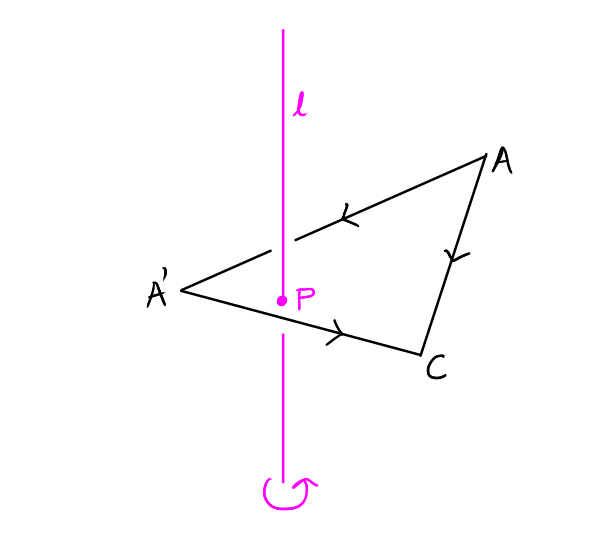
\includegraphics[scale=.25]{images/1.png}
\end{center}
Since there are finitely many edges in $L$, this process stops with all edges winding counterclockwise. Then we draw a radial line from $P$ intersecting the edges transversely at finitely many points. From this we get a braid; the points of intersection give the endpoints of the braid.

\subsection{Yamada-Vogel algorithm}

The original proof of Alexander's theorem was algorithmic, that is, it gave an algorithm for transforming a knot or link into closed braid form. Despite the simplicity and the straightforwardness of the proof, it is difficult and impractical to write a computer program based upon it. We shall see a different proof originally due to Yamada but improved later by Vogel. This proof has two major advantages: (1) We can write an efficient computer program for putting knots or links in closed braid form; (2) It has a beautiful corollary that reveals structure about link diagrams.

The Yamada-Vogel algorithm is based on Seifert's algorithm for constructing a Seifert surface for an oriented knot or link $K$. First, we need some definitions and terminology.

Seifert's algorithm on an oriented link diagram involves smoothing all crossings of a given oriented link in the standard orientation-preserving way. This yields a disjoint union of oriented loops (topological circles) called \emph{Seifert cirlces}. We observe that any two disjoint oriented (topological) circles on the sphere $S^2$ bound an annulus in $S^2$. These circles are said to be \emph{incompatible} if their orientation is induced by an orientation of this annulus. Otherwise, these circles are \emph{compatible}. For instance, two oriented concentric cirles in $\R^2$
are compatible if they both are oriented clockwise or both counterclockwise.

The number of Seifert circles of an oriented link diagram $D$ is denoted by $n(D)$. Two Seifert circles of an oriented link diagram $D$ are said to be \emph{compatible} (resp. \emph{incompatible}) if they are compatible (resp. incompatible) in $S^2 = \R \cup \{ \infty \}$. The number of pairs of incompatible Seifert circles of $D$ is denoted by $h(D)$ and is called the \emph{height} of $D$. 

Let $|D| \in \R^2$ be the 4-valent graph we get from $D$ with the over/undercrossing data forgotten. The vertices are then the crossings of $D$. An \emph{edge} of $D$ is defined in the obvious way considering $|D|$ as a planar graph. Edges of $D$ are then arcs or circles in $\R^2$. A \emph{face} of $D$ is also defined in the obvious way. A face $f$ of $D$ is said to be \emph{adjacent} to an edge $e$ of $D$ if $e$ is contained in the closure of $f$, that is, $e$ forms a boundary of $f$. A face $f$ is said to be \emph{adjacent} to a Seifert circle $S$ of $D$ if $f$ is adjacent to at least one edge of $D$ contained in $S$. A face $f$ of $D$ is said to be a \emph{defect face} if $f$ is adjacent to distinct edges $e_1, e_2$ of $D$ such that the Seifert circles $S_1, S_2$ of $D$ going along $e_1, e_2$ are distinct and incompatible. An oriented arc $c \subset \R^2$ leading from a point of edge $e_1$ to a point of edge $e_2$ and lying (except the endpoints) in $f$ is called a \emph{reduction arc} of $D$ in $f$. A Yamada-Vogel reducing move, denoted by $\mathcal{Y}$ (or $\mathcal{Y}^+$), on two arcs $a_1, a_2$ belonging to two distinct incompatible Seifert circles is the following:

\begin{center}
  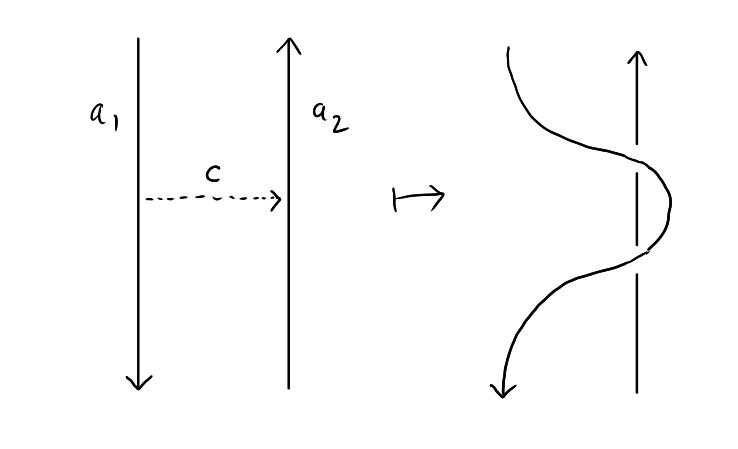
\includegraphics[scale=.25]{images/2.png}
\end{center}
The inverse of the Yamada-Vogel reducing move is denoted by $\mathcal{Y}^-$. With this, we are ready to write and prove the following three lemmas.

\begin{lemma}
    \label{l1}
If $D^{\prime}$ is obtained from an oriented link diagram $D$ in $\mathbb{R}^2$ by a reducing move, then $n(D^{\prime}) = n(D)$ and $h(D^{\prime}) = h(D) - 1$.
\end{lemma}

\begin{proof}
  Suppose that $S_1, S_2$ are two distinct and incompatible Seifert circles of $D$ involved in the Yamada-Vogel reducing move $\mathcal{Y}$ (shown in the figure). The move gives rise to two new Seifert circles $S_0$ and $S_{\infty}$. It is easy to see that all other Seifert circles of $D$ are left untouched. The first part of the lemma follows. We note that Seifert circles of $D$ and $D^{\prime}$ do not pass through the shaded areas in the figure.

\begin{center}
 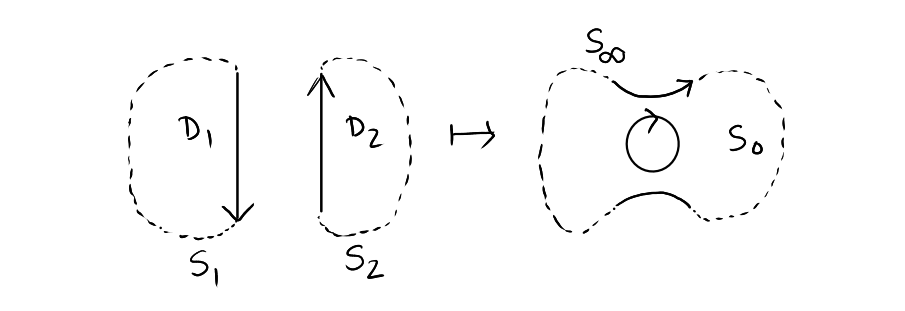
\includegraphics[scale=.25]{images/3.png}
\end{center}
  
  Let $D_1, D_2$ be the disjoint disks bounded by the Seifert circles $S_1, S_2$. Let $d_i$ denote the number of Seifert circles of $D$ lying in the open disk $D_i^{\circ} = D_i - \partial D_i$. Let $d$ be the number of Seifert circles of $D$ lying in the annulus $S^2 - (D_1 \cup D_2)$ and incompatible with $S_1$. Let $h$ be the number of pairs of incompatible Seifert circles of $D$ both distinct from $S_1, S_2$. We claim that $h(D) = h + d_1 + d_2 + 2d + 1$. It suffices to check that the number of pairs of incompatible Seifert circles of $D$ including $S_1$ or $S_2$ or both is equal to $d_1 + d_2 + 2d + 1$. For $i = 1, 2$, an oriented circle in $D_i^{\circ}$ is incompatible with $S_1$ or $S_2$, but not with both. This gives the contribution $d_1 + d_2$. An oriented circle in $S^2 - (D_1 \cup D_2)$ is incompatible with $S_1$ if and only if it is incompatible with $S_2$. This contributes $2d$. Finally, $S_1$ and $S_2$ are incompatible, which contributes $1$.

  We claim that $h(D^{\prime}) = h + d_1 + d_2 + 2d = h(D) - 1 $. We simply check that the number of pairs of incompatible Seifert circles of $D^{\prime}$ including $S_0$ or $S_{\infty}$ or both is equal to $d_1 + d_2 + 2d$. A similar argument checks this. Hence $h(D^{\prime}) = h(D) - 1$.
\end{proof}

\begin{lemma}
  \label{l2}
An oriented link diagram $D$ in $\mathbb{R}^2$ has a defect face if and only if $h(D) \ne 0$.
\end{lemma}

\begin{proof}
  Let $\Sigma$ denote the compact surface with boundary we obtain by cutting $S^2$ open along the Seifert circles of $D$. For a crossing $x$ of $D$, let $\gamma_x$ denote a line segment near $x$ joining the Seifert circles (shown in the figure). These line segments are all disjoint with each of them lying in a component of $\Sigma$.

\begin{center}
 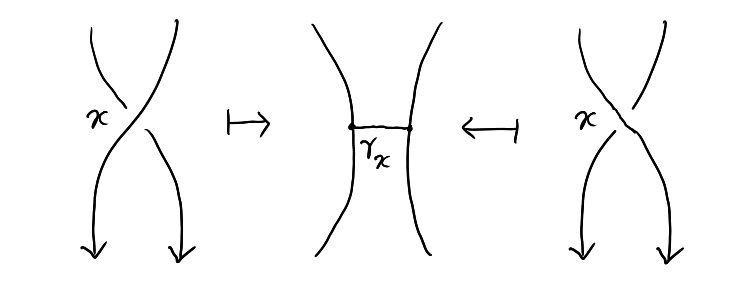
\includegraphics[scale=.25]{images/4.png}
\end{center}
  
  The forward direction of the lemma is obvious from the definition of a defect face. Therefore, we only prove that if $h(D) > 0$, then $D$ has a defect face. First, we prove that there are a component $F$ of $\Sigma$ and two Seifert circles in $\partial F$ whose orientation is induced by an orientation on $F$. Pick two incompatible Seifert circles $S_1, S_2$ of $D$ and consider an oriented arc $c \subset \R^2$ leading from a point of $S_1$ to a point of $S_2$. We can assume that $c$ meets each Seifert circle of $D$ transversely in at most one point. The crossings of $c$ with these circles form a finite subset of $c$ including the endpoints. At each of the crossings, the corresponding Seifert circle is directed to the left or to the right of $c$. The incompatibility of $S_1, S_2$ means that their directions at the endpoints of $c$ are opposite: one of these circles is directed to the left of $c$ and the other one is directed to the right of $c$. Therefore, among the crossings of $c$ with the Seifert circles of $D$, there are two that lie consecutively on $c$ and at which the directions of the corresponding
  Seifert circles are opposite. The component $F$ of $\Sigma$ containing the subarc of $c$ between two such crossings satisfies the requirements above.

  Consider a component $F$ of $\Sigma$ such that there are at least two Seifert circles in $\partial F$ whose orientation is induced by an orientation on $F$. We fix such an orientation on $F$. We call a Seifert circle in $\partial F$ positive if its orientation is induced by the one on $F$ and negative otherwise. By assumption, there are at least two positive Seifert circles in $\partial F$. If $F$ contains no segments $\gamma_x$, then $F^{\circ} = F - \partial F$ is a face of $D$ adjacent to $\geq 2$ positive Seifert circles in $\partial F$. Hence this face is a defect face. Suppose that $F$ contains certain segments $\gamma_x$. Removing them all from $F$, we obtain a subsurface $F^{\prime}\subset F$. It is clear that any component $f$ of $F^{\prime}$ is adjacent to at least one segment $\gamma_x$ and the interior of $f$ is a face of $D$. Each $\gamma_x \subset F$ connects a positive Seifert circle in $\partial F$ with a negative one. Therefore $f$ is adjacent to at least one positive and at least one negative Seifert circle. If $f$ is adjacent to at least two positive or to at least two negative Seifert circles, then $f$ is a defect face. Suppose that each component $f$ of $F^{\prime}$ is adjacent to exactly one positive and exactly one negative Seifert circle. Note that moving from $f$ to a neighboring component of $F^{\prime}$ across some $\gamma_x\subset F$, we meet the same Seifert circles. Since $F$ is connected,
we can move in this way from any component of $F^{\prime}$ to any other component. Therefore $\partial F$ contains exactly one positive and one negative Seifert circle. This contradicts our assumptions. Hence $D$ has a defect face.
\end{proof}

\begin{lemma}
\label{l3}
An oriented link diagram $D$ in $\mathbb{R}^2$ with $h(D) = 0$ is isotopic in the sphere $S^2 = \mathbb{R}^2 \cup \{\infty\}$ to a closed braid diagram in $\mathbb{R}^2$.
\end{lemma}

\begin{proof}
  Suppose that $h(D) = 0$. We are to prove that $D$ is isotopic in $S^2$ to a closed braid diagram in $\R^2 = S^2 - \{\infty\}$. If a certain component
of the surface $\Sigma$ has three or more boundary components, then two of them
must be incompatible in $S^2$, which contradicts our assumption $h(D) = 0$.

  We observe that a compact connected subsurface of the 2-sphere whose boundary has at most two components is either a disk or an annulus. Therefore, $\Sigma$ consists only of disks and annuli. An induction on the number of annuli components of $\Sigma$ shows that the Seifert circles of $D$ can be transformed by an isotopy of $S^2$ into a union of disjoint concentric circles in $\R^2$. If we apply this isotopy of $S^2$ to $D$, we can assume from the very beginning that the Seifert circles of $D$ are concentric circles in the plane. The equality $h(D) = 0$ implies that all these circles are oriented
in the same direction, either clockwise or counterclockwise. In the first case we apply to $D$ an additional isotopy pushing all its Seifert circles across infinity so that in the final position the Seifert circles of $D$ become concentric circles in $R^2$ with counterclockwise orientation. With a further isotopy of $D$, we can additionally ensure that these circles are concentric Euclidean circles and the segments $\gamma_x$ are radial, i.e., are contained in some radii. The resulting link diagram is transversal to all radii and therefore is a closed braid diagram.
\end{proof}

The algorithm is now immediate. To transform any diagram $D$ of an oriented link $K$ in $\R^3$ into a closed braid diagram of $K$, it suffices to perform the reducing move on the diagram each time there is a defect face. By Lemmas \ref{l1} and \ref{l2}, this process should stop after $h(D)$ steps yielding a diagram $D^{\prime}$ of $L$ with $n(D^{\prime}) = n(D)$ and $h(D^{\prime}) = 0$. But then $D^{\prime}$ is isotopic in $S^2$ to a closed braid diagram in $\R^2$. 

\begin{definition}
  The braid index of a link $K$ is the minimum number $n$ such that there exists a braid $\beta \in B_n$ whose closure $\bar{\beta}$ represents $K$.
\end{definition}

As pointed out earlier, the Yamada-Vogel algorithm has the corollary:
  
\begin{corollary}
  The minimum number of Seifert circles in any diagram of a link $K$ is equal to the braid index of $K$.
\end{corollary}

\begin{proof}
This follows from the algorithm since $n = n(D)$ is unchanged. The converse is obvious.
\end{proof}

\begin{corollary}
Let $N$ denote the length of any sequence of reducing moves required to transform a diagram $D$ into closed braid form. Then 
\begin{displaymath}
N = h(D) \leq \frac{(n-1)(n-2)}{2}.
\end{displaymath}
\end{corollary}

\section{Markov's Theorem}
\label{Markov}

\subsection{Markov's theorem}

Alexander's theorem guarantees that any oriented link can be realized as a closed braid. But it has no say on the uniqueness of the closed braid and as such, it has little use in studying knots from braid groups. Markov's theorem states that any two braids expressing the same link are mutually related by successive applications some special moves, which we describe below.

Let $\beta \in \B_n$ be a braid. A Markov move is defined to be any one of the following types
\begin{enumerate}
\item\label{item:6} Conjugation: Transforming $\beta \to \alpha \beta \alpha^{-1}$ or inverse,
\item\label{item:10} The move $\beta \to \beta \sigma_n^{\pm 1}$ where $\beta \in B_n$ and $\beta \sigma_n^{\pm 1} \in B_{n+1}$,
\item\label{item:12} Isotopy in the given Artin braid group.
\end{enumerate}
\begin{theorem}[Markov]
    Two braids have isotopic closures in $\mathbb{R}^3$ if and only if these braids are related by a sequence of Markov moves.
  \end{theorem}
  The theorem can also be formulated in the following way:
\begin{theorem}[Markov]
\label{sec:markovs-theorem}
  Let $Y$, $Y^{\prime}$ be closed braid representatives of the same oriented link $K$ in $\R^3$. Then there exists a sequence of closed braid representatives of $K$: 
\begin{displaymath}
Y = Y_1 \to Y_2 \to \cdots \to Y_r = Y^{\prime}
\end{displaymath}
such that each $Y_{i+1}$ is obtained from $Y_i$ by a single Markov move.
\end{theorem}

We say that two closed braids are Markov-equivalent or M-equivalent if they are related by a sequence of Markov moves. To prove this theorem, we use (without proof) the well-known Reidemeister's theorem.

Given closed braids $Y$ and $Y^{\prime}$ which represent the same oriented link $K$, we may assume that $h(Y) = h(Y^{\prime}) = 0$. By Reidemeister's theorem, there is a sequence of knot diagrams $Y = Y_1 \to Y_2 \to \cdots \to Y_r = Y^{\prime}$, where $h(Y_i) \geq 0$ for $i = 2,\ldots,k-1$, such that any two diagrams in the sequence are related by a single Reidemeister move.

\begin{lemma}
It suffices to prove Markov's theorem for closed braids $Y, Y^{\prime}$ which are related by sequences $Y = Y_1 \to Y_2 \to \cdots \to Y_q = Y^{\prime}$ with the properties (i) $h(Y) = h(Y^{\prime}) = 0$, (ii) $h(Y_i) > 0$ for $i = 2, \ldots, q-1$, and (iii) $Y_{i+1}$ is obtained from $Y_i$ by a single $\mathcal{Y}^{\pm}$.
\end{lemma}
\begin{proof}
  We may always assume that the diagrams $Y_2, \ldots, Y_q$ have height $> 0$, for if not we simply replace the given sequences by the subsequences joining any two intermediate diagrams of height zero.
  
  A Reidemeister move is said to be braid-like if the strands that are involved in it have same orientation locally. It is clear that any Reidemeister move of type I is already braid-like. First we claim that we can get from $Y$ to $Y^{\prime}$ via a finite sequence of the following four types of moves and their inverses: 
\begin{enumerate}
\item\label{item:1} Braid-like Reidemeister move of type I, denoted by I$^b$, 
\item\label{item:2} Braid-like Reidemeister move of type II, denoted by II$^b$,
\item\label{item:3} Braid-like Reidemeister move of type II, denoted by III$^b$,
\item\label{item:4} Yamada-Vogel reducing move $\mathcal{Y}$.
\end{enumerate}

To prove this claim, it suffices to show that all the non-braid-like Reidemeister moves, denoted by I$^{nb}$, II$^{nb}$ and III$^{nb}$, can be achieved via a finite sequence of moves to type I$^b$, II$^{b}$, III$^b$ and $\mathcal{Y}$. 
\begin{enumerate}
\item\label{item:5} As noted above, any type I Reidemeister move is of type I$^n$. 
\item\label{item:11} Since there are three arcs involved in type III Reidemeister move, there are several different cases to check. One possible case in given in the diagram below.

\begin{center}
 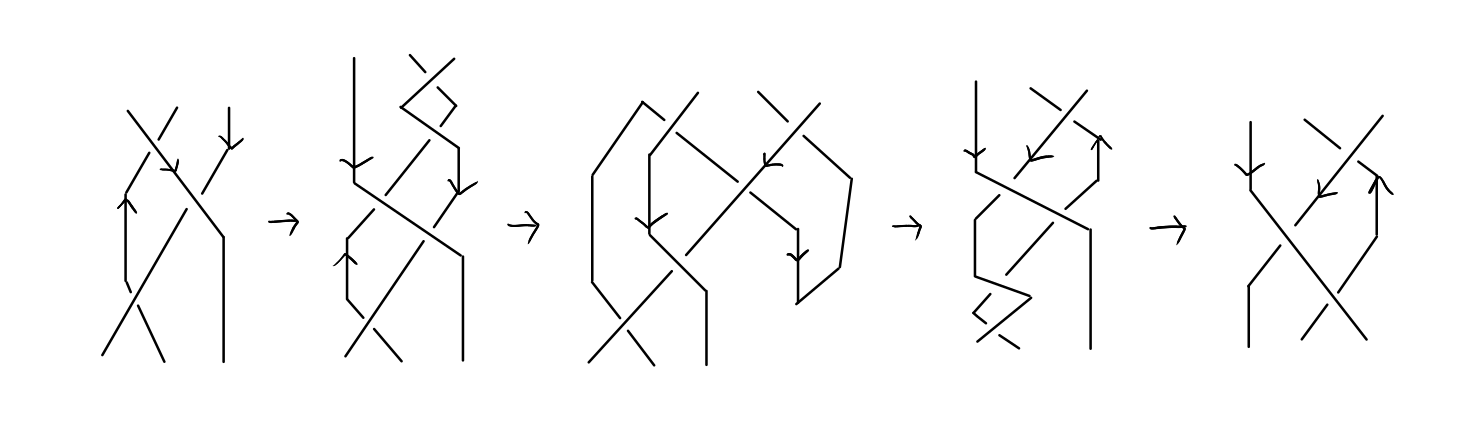
\includegraphics[scale=.25]{images/5.png}
\end{center}

The replacement sequence shows that this case of II$^{nb}$ can be achieved
by a sequence consisting of a type II$^{nb}$ move, an isotopy, a type III$^b$ move and finally another type II$^{nb}$ move. Other cases of III$^{nb}$ can be similarly checked.
\item\label{item:15} A move of II$^{nb}$ may be regarded as $\mathcal{Y}^{\pm}$ if the arcs involved belong to distinct Seifert circles. If they belong to the same Seifert circle, the move can be achieved as a sequence of two moves of I$^b$, a move of $\mathcal{Y}$ and a move of $\mathcal{Y}^{-}$. This is shown in the diagram below.
\begin{center}
 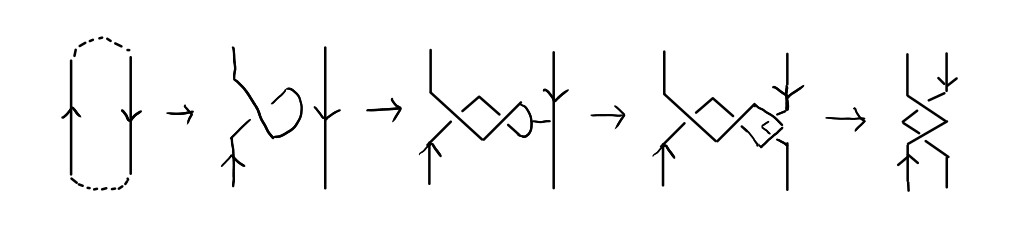
\includegraphics[scale=.25]{images/6.png}
\end{center}
\end{enumerate}
Further it can be shown that the braid-like Reidemeister moves can be achieved via Markov moves and $\mathcal{Y}^{\pm}$.

By doing this, we have thus replaced our original sequence relating $Y$ to $Y^{\prime}$ by a new one which is in general much longer, but which consists entirely of Markov moves (performed, by definition, on braid diagrams, i.e., on diagrams of height zero) and moves of type $\mathcal{Y}^{\pm}$. To be precise, our original sequence from $Y$ to $Y^{\prime}$ may be replaced by a sequence of the form $Y = Y_0,\ldots, Y_{a_1},\ldots, Y_{a_2},\ldots, Y_{a_n} = Y^{\prime}$, where $h(Y_{a_i}) = 0$ for all $i$ and in each subsequence $Y_{a_i},\ldots,Y_{a_{i+1}}$, either (1) each diagram in the subsequence has height zero and adjacent diagrams are related by a single Markov move, or (2) all the intermediate diagrams have strictly positive height and adjacent diagrams are related by a single move of type $\mathcal{Y}^{\pm}$.
\end{proof}

We have eliminated Redeimeister moves completely. We started with a sequence relating the given braids $Y$ and $Y^{\prime}$ that consisted entirely of Reidemeister moves. We replaced it with a sequence of reducing moves and braid-like Reidemeister moves. The latter are in general not applied to
diagrams of height zero, but we changed them to apply to diagrams of height zero. That is the moment when braid-like Reidemeister moves were changed to Markov moves.

Consider the graph of the height function on our sequence. We will examine local maxima in the height function. Let $Y(r), \hat{Y}, Y(s)$ be three consecutive diagrams in our sequence such that the height function has a local maximum at $\hat{Y}$. We have two reducing moves $r,s $ with corresponding arcs $\alpha_r, \alpha_s$ in $\hat{Y}$ such that reducing $\hat{Y}$ along $\alpha_r$ (resp. $\alpha_s$) results in the diagram $Y(r)$ (resp. $Y(s)$). Such a triple  $\{Y(r), \hat{Y}, Y(s)\}$ such that the height function has a local maximum at $\hat{Y}$ is called a peak. The height of the peak is defined to be $h(\hat{Y})$ and height of the sequence is defined to be the maximum over the height of all the peaks in the sequence. 

We may assume that the reducing arcs involved in any peak are disjoint. Further, the adjustments in our sequence of reducing moves which are required preserve the height of the sequence. When the reducing arcs involved in a peak $\{Y(r), \hat{Y}, Y(s) \}$ are disjoint, the reducing moves commute, that is, they can be performed in either order, starting with the diagram $\hat{Y}$ and resulting in the same diagram $Y^{\prime}$. Further, as long as the
reducing arcs $\alpha_r, \alpha_s$ act on $3$ or $4$ distinct Seifert circles, we can perform the two reducing moves in either order with the same result. In
this case we say we have a ‘commuting pair’ of reducing moves associated to the peak. If a peak $\{Y(r), \hat{Y}, Y(s) \}$ has a commuting pair, then we may replace it by a ‘valley’, that is, a subsequence $\{Y(r), Y^{\prime}, Y(s) \}$ where $h(Y^{\prime}) = h(Y) - 2$ and $Y^{\prime} = Y(s \circ r) = Y(r \circ s)$ is the result of reducing $Y(r)$ along $\alpha_s$, or equivalently reducing $Y(s)$ along $\alpha_r$. Thus we can eliminate any peak corresponding to a commuting pair (such a peak necessarily has height at least 2).

If the two reducing arcs at a peak act on the same 2 circles, then after one move is performed, the second Reidemeister move will no longer be a reducing move; we call this a ‘non-commuting pair’ of reducing moves. Let $\{Y(r), \hat{Y}, Y(s) \}$ be a peak corresponding to a non-commuting pair of reducing arcs, and let $C_1, C_2$ be the two Seifert circles involved. Suppose there is a reducing arc $\alpha_t$ such that $\alpha_t$ is non-intersecting with $\alpha_r$ and $\alpha_s$, and such that $t$ involves a circle other than $C_1$ or $C_2$, then we can insert $t$ at $Y^{\prime}$ to replace our peak $\{Y(r), \hat{Y}, Y(s) \}$  with two new peaks with commuting pairs of reducing moves: $\{Y(r), Y^{\prime}, Y(t)\}$ and $\{Y (t), \hat{Y}, Y (s)\}$.
As above, we now replace each peak with a ‘valley’: ${Y (r), Y^{\prime}, Y (t)}$ and ${Y (t), Y^{\prime\prime}, Y (s)}$, respectively, where $Y^{\prime}= Y (t \circ r) = Y (r \circ t)$ is the diagram resulting from reducing $Y(r)$ by
$t$ (or equivalently, from reducing $Y(t)$ by $r$, and $Y^{\prime\prime}$ is the diagram resulting from reducing $Y(s)$ by $t$ (or equivalently, from reducing $Y(t)$ by $s$). Again, this implies that the height of the original non-commuting peak $\{Y (r), \hat{Y}, Y (s)\}$ was at least 2. Thus, we can replace such a peak with peaks of strictly smaller height and repeat this process until all peaks either have height 1 or do not admit such a reducing arc $\alpha_t$ as above; we call a peak of the latter type irreducible.

We may assume that any peak in the height function of our sequence either
has height 1 or is irreducible. This is clear from our discussion above.

\begin{lemma}
\label{sec:markovs-theorem-2}
We may assume that no peaks in the height function of our sequence have
height 1.
\end{lemma}

\begin{proof}
\label{sec:markovs-theorem-3}
Let $\{Y(r), \hat{Y}, Y(s)\}$ be a peak of height 1. See that height 1 implies that the two reducing arcs are non-commutative and hence involve precisely two circles. It is an easy exercise to show that these two circles must live either on the ‘inside’ or on the ‘outside’ of a band of circles, and that $\alpha_r$ and $\alpha_s$ are in fact equivalent as reducing moves.
Therefore the diagram $Y(r)$ is equivalent to $Y(s)$ and we can simply eliminate this peak from our sequence.
\end{proof}

A Seifert circle with weight $w$ attached means a collection of $w$ compatible, nested, parallel Seifert circles. We use the term band for a Seifert circle with an attached weight.

\begin{lemma}
  \label{ulem1}
  If $\{Y(r), \hat{Y}, Y(s) \}$ is a irreducible peak in the height function of our sequence, then the diagram $\hat{Y}$ contains at most four bands, arranged as in the following figure.
\end{lemma}
\begin{center}
 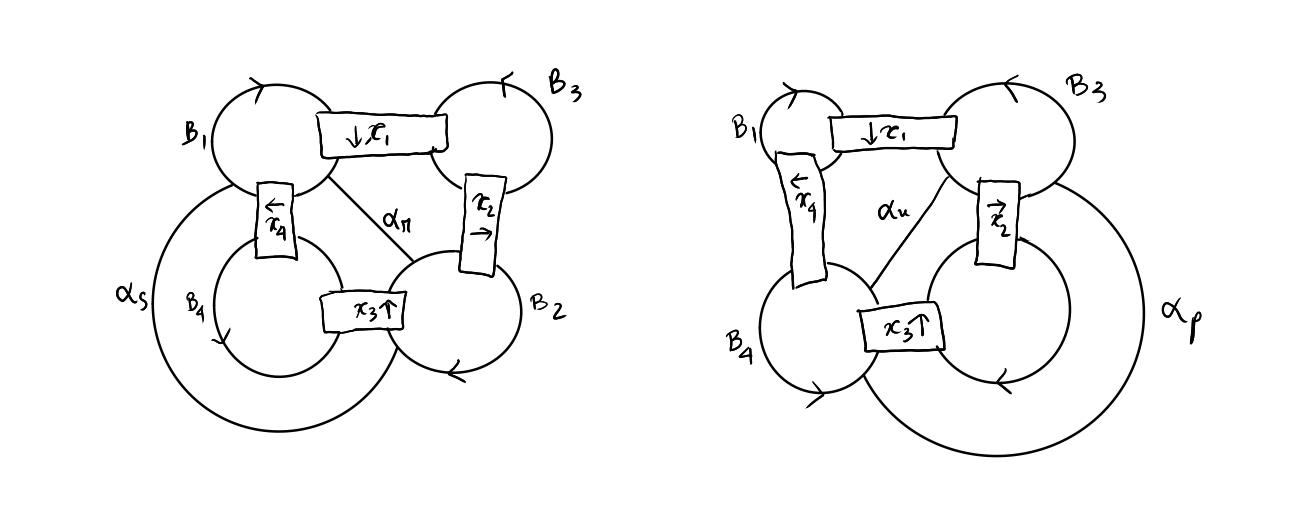
\includegraphics[scale=.25]{images/7.png}
\end{center}

  \begin{lemma}
   \label{ulem2}
 Let $\{ Y(r), \hat{Y}, Y(s)\}$ be an irreducible peak of height $n+1$ in the height function of our sequence. Then there exist sequences of diagrams $Y(r) = Y_1^r, \ldots, Y_n^r = Y(p \circ r)$ and $Y(s) = Y_1^s, \ldots, Y_n^s = Y (u \circ s)$ such that $Y^r_{i+1} $ (resp. $Y^s_{i+1}$) is obtained from $Y_i^r$ (resp. $Y_i^s$) by a reducing move and such that $h(Y(p \circ r)) = h(Y(u\circ s)) = 0$ and $Y(p\circ r) = 0$ and $Y(p \circ r) $ and $Y(u \circ s))$ are Markov equivalent.
   \end{lemma}

The proofs of Lemmas \ref{ulem1} and \ref{ulem2} can be found in \cite{Bsurvey}.

  We have already reduced the proof to the situation of two closed braid diagrams $Y$ and $Y^{\prime}$ related by a sequence of diagrams related by reducing moves (and their inverses) such that the height of each intermediate diagram is strictly positive and such that any peak in the height function of the sequence is irreducible (of height at least 2). Let $\{ Y(r), \hat{Y}, Y(s)\}$ be an irreducible peak of height $n$ in the height function of our sequence. By previous lemma, we can replace this subsequence with a subsequence of strictly smaller height. In doing so, we create new peaks whose height is strictly lower than the height of the peak being replaced. If we perform this operation at every irreducible peak, then we obtain a new
sequence relating our closed braid diagrams $Y, Y^{\prime}$. By induction on the height of the sequence, we can replace any sequence with a sequence consisting entirely of diagrams of height zero.

\subsection{Markov functions}

Markov's theorem gives us a tool to construct invariants for knots and links. Here we define Markov functions and show how link invariants can be constructed.

  \begin{definition}
  A Markov function with values in a set $E$ is a sequence of set-theoretic maps $\{ f_n: B_n \to E \}_{n\geq 1}$, satisfying the following conditions: 
\begin{enumerate}
\item\label{item:13} for all $n \geq 1$ and all $\alpha, \beta \in B_n$, 
\begin{displaymath}
f_n(\alpha \beta ) = f_n (\beta \alpha);
\end{displaymath} 
\item\label{item:14} for all $n \geq 1$ and all $\beta \in B_n$, 
\begin{displaymath}
f_n(\beta) = f_{n+1}(\sigma_n \beta) \text{ and } f_n(\beta) = f_{n+1}(\sigma_n^{-1} \beta).
\end{displaymath}
\end{enumerate}
\end{definition}

\begin{theorem}
  \label{markovisotopy}
  Any Markov function $\{ f_n : B_n \to E \}_{n \geq 1}$ determines an $E$-valued isotopy invariant $\hat{f}$ of oriented links in $\mathbb{R}^3$.
\end{theorem}
\begin{proof}
  Let $K$ be an oriented link in $\mathbb{R}^3$. Pick a braid $\beta \in B_n$ whose closure is isotopic to $K$ and set $\hat{f}(K) = f_n(\beta) \in E$. Check that $\hat{f}(K)$ does not depend on the choice of $\beta$. Indeed, if $\beta^{\prime} \in B_{n^{\prime}}$ is another braid whose closure is ambient isotopic to $K$, then $\beta$ and $\beta^{\prime}$ are M-equivalent (by Markov's theorem). It can be seen from M-equivalence and the definition of the Markov function that $f_n(\beta) = f_{n^{\prime}}(\beta^{\prime})$. The function $\hat{f}$ is an isotopy invariant of oriented links: if $K, K^{\prime}$ are isotopic oriented links in $\mathbb{R}^3$ and $\beta \in B_n$ is a braid whose closure is isotopic to $K$, then the closure of $\beta$ is also isotopic to $K^{\prime}$ and $\hat{f}(K) = f_n(\beta) = \hat{f}(K^{\prime})$.
\end{proof}

\section{Representation of Braid Groups}
\label{Burau}

\subsection{Burau representation}

  Fix $n\geq 2$. For $i=1,2,\ldots, n-1$, define 
\begin{displaymath}
  U_i = \begin{pmatrix} I_{i-1} & 0 & 0 & 0 \\
    0 & 1-t & t & 0 \\
    0 & 1 & 0 & 0 \\
  0 & 0 & 0 & I_{n-i-1}\end{pmatrix}.
\end{displaymath}
  Since $U_i$ are invertible, $U_i \in \text{GL}_n(\Uplambda)$, where $\Uplambda = \mathbb{Z}[t, t^{-1}]$ is the ring of Laurent polynomials.

    Since $U_i$ have block form, it is easy to check that
\begin{align*}
  U_iUj &= U_jU_i \hspace*{4em}\text{for }|i-j| > 1 \\
  U_iU_{i+1}U_i &= U_{i+1}U_iU_{i+1}.
\end{align*}
To check the last equation, it suffices to show that 
\begin{displaymath}
\begin{pmatrix} 1-t & t & 0 \\ 1 & 0 & 0 \\ 0 & 0 & 1 \end{pmatrix}
  \begin{pmatrix} 1 & 0 & 0 \\ 0 & 1-t & t \\ 0 & 1 & 0 \end{pmatrix}
  \begin{pmatrix} 1-t & t & 0 \\ 1 & 0 & 0 \\ 0 & 0 & 1 \end{pmatrix} =
  \begin{pmatrix} 1 & 0 & 0 \\ 0 & 1-t & t \\ 0 & 1 & 0 \end{pmatrix}
  \begin{pmatrix} 1-t & t & 0 \\ 1 & 0 & 0 \\ 0 & 0 & 1 \end{pmatrix}
  \begin{pmatrix} 1 & 0 & 0 \\ 0 & 1-t & t \\ 0 & 1 & 0 \end{pmatrix}
\end{displaymath}
  Since $U_i$ satisfy the braid relations, we have a group homomorphism 
\begin{align*}
\label{eq:1}
  \psi_n : B_n &\to \text{GL}_n(\Uplambda) \\
  \sigma_i &\rightsquigarrow U_i.
\end{align*}
This is the Burau representation of the Artin braid group $B_n$.

We observe that $\det(U_i) = -t$ for all $i$. This implies that for any $\beta \in B_n$, 
\begin{displaymath}
\det \psi_n(\beta) = (-t)^{\langle \beta \rangle}
\end{displaymath}
where $\langle \beta \rangle \in \Z$ is the image of $\beta$ under the homomorphism $B_n \to \Z$ sending the generators $\sigma_1, \ldots, \sigma_{n-1}$ to $1$.

The Burau representations $\{ \psi_n \}_{n\geq 1}$ are compatible with the natural inclusions $\iota : B_n \hookrightarrow B_{n+1}$: for any $n\geq 1 $ and $\beta \in B_n$, 
\begin{equation}
\label{eq:3}
\psi_{n+1}(\iota(\beta)) = \begin{pmatrix} \psi_n(\beta) & 0 \\ 0 & 1 \end{pmatrix}.
\end{equation}

Now we show that the Burau representation is reducible. For $n\geq 3$, we define the following $(n-1)\times(n-1)$ matrices 
\begin{displaymath}
  V_1 = \begin{pmatrix} -t & 0 & 0 \\ 1 & 1 & 0 \\ 0 & 0 & I_{n-3} \end{pmatrix},
  V_i = \begin{pmatrix} I_{i-1} & 0 & 0 & 0  & 0 \\ 0 & 1 & t & 0 & 0 \\ 0 & 0 & -t & 0 & 0 \\0 & 0 & 1 & 1 & 0 \\ 0 & 0 & 0 & 0 & I_{n-i-2} \end{pmatrix},
  V_{n-1} = \begin{pmatrix} I_{n-3} & 0 & 0 \\ 0 & 1 & 1 \\ 0 & 0 & -t \end{pmatrix},
\end{displaymath}
where $i = 1, \ldots, n-1,$. Let $C$ be the $n\times n$ matrix 
\begin{displaymath}
C = C_n = \begin{pmatrix} 1 & 1 & 1 & \cdots & 1 \\ 0 & 1 & 1 & \cdots &  1 \\ 0 & 0 & 1 & \dots & 1 \\ \cdot & \cdot & \cdot & & \cdot \\ 0 & 0 & 0 & \cdots & 1\end{pmatrix}.
\end{displaymath}
Then we have the following result:

\begin{theorem}
\label{sec:burau-representation}
Let $*_i$ be the row of length $n-1$ equal to $0$ if $i<n-1$ and to $\begin{pmatrix} 0 & 0 & \cdots & 0 & 1 \end{pmatrix}$ if $i = n-1$. Then 
\begin{equation}
\label{eq:6}
C^{-1} U_i C = \begin{pmatrix} V_i & 0 \\ *_i & 1 \end{pmatrix}.
\end{equation}
\end{theorem}

\begin{proof}
\label{sec:burau-representation-1}
For $i=1, \ldots, n-1$, we set 
\begin{displaymath}
  V_i^{\prime} = \begin{pmatrix} V_i & 0 \\ *_i & 1 \end{pmatrix}.
\end{displaymath}
It suffices to show that $U_iC = CV_i^{\prime}$ for all $i$. We fix $i$ and observe that for any $k= 1, \ldots, n$, the $k$th column of $U_iC$ is the sum of the first $k$ columns of $U_i$. A direct computation shows that $U_iC$ is obtained from $C$ by replacing the $(i, i)$th entry by $1-t$ and replacing the $(i+1, i)$th entry by $1$. Similarly, for any $l = 1, \ldots, n$, the $l$th row of $CV_i^{\prime}$ is the sum of the last $l$ rows of $V_i^{\prime}$. A direct computation shows that $CV_i^{\prime}$ is obtained from $C$ by the same modification as above. Hence $U_iC = CV_i^{\prime}$.
\end{proof}

Since $U_i$ satisfy the braid relations, $C^{-1}U_iC$ also satisfy them. Using the formula (\ref{eq:6}), it is easily checked that $V_i$ also satisfy the braid relations. Also, $V_i \in \text{GL}_{n-1}(\Uplambda)$.

We have the reduced Burau representation, for $n\geq 3$
\begin{align*}
  \psi^r_n: B_n &\to \text{GL}_{n-1}(\Uplambda) \\
  \sigma_i &\rightsquigarrow V_i.
\end{align*}
  For $n=2$, we define 
\begin{align*}
  \psi^r_2 : B_2 &\to \text{GL}_{1}(\Uplambda) \\
  \sigma_1 &\rightsquigarrow (-t),
\end{align*}
which is chosen so that the formula (\ref{eq:6}) holds for $n=2$. This formula implies that for any $n\geq 2$ and any braid $\beta \in B_n$, 
\begin{equation}
\label{eq:5}
C^{-1} \psi_n(\beta) C = \begin{pmatrix} \psi_n^r(\beta) & 0 \\ *_{\beta} & 1 \end{pmatrix},
\end{equation}
where $*_{\beta}$ is a row of length $n-1$ over $\Z[t, t^{-1}]$ depending on $\beta$. The following lemma shows how to compute this row from the matrix $\psi_n^r(\beta)$.

\begin{lemma}
\label{sec:burau-representation-3}
For $i = 1, \ldots, n-1$, let $a_i$ be the $i$th row of the matrix $\psi_n^r(\beta ) - I_{n-1}$. Then 
\begin{displaymath}
-(1 + t + \cdots + t^{n-1})*_{\beta} = \sum_{i=1}^{n-1} (1+ t + \cdots + t^i)a_i.
\end{displaymath}
\end{lemma}

\begin{proof}
\label{sec:burau-representation-4}
Consider the $\Uplambda$-module $\Uplambda^n$. The elements are rows of length $n$ over $\Uplambda$. The group $GL_n(\Uplambda)$ acts on $\Uplambda^n$ on the right via the multiplication of rows by matrices. It can be directly verified that the vector 
\begin{displaymath}
E = (1, t, t^2, \ldots, t^{n-1}) \in \Uplambda^n
\end{displaymath}
satisfies $EU_i = E$ for all $i$. Hence, $E\psi_n(\beta) = E$. Then the vector 
\begin{displaymath}
F = EC = (1, 1 + t, 1 + t + t^2, \ldots, 1 + t + \cdots + t^{n-1}) \in \Uplambda^n
\end{displaymath} satisfies 
\begin{displaymath}
F \begin{pmatrix} \psi_n^r(\beta) & 0 \\ *_{\beta} & 1 \end{pmatrix} = ECC^{-1}\psi_n(\beta) C = EC = F.
\end{displaymath}
Subtracting $FI_n = F$, it follows that 
\begin{displaymath}
F \begin{pmatrix} \psi_n^r(\beta) - I_{n-1} \\ *_{\beta} \end{pmatrix} = 0.
\end{displaymath}
This equality means that the linear combination of the rows $a_i$ of the matrix $\psi_n^r(\beta) - I_{n-1}$ with coefficients $1, 1+t, 1 + t + t^2, \ldots, 1 + t + \cdots + t^{n-2}$ is equal to $-(1 + t + \cdots + t^{n-1})*_{\beta}$.
\end{proof}

% This lemma makes it clear that we lose no information when we pass from the Burau representation to its reduced form. 

\subsection{Alexander-Conway polynomial}

Let $g: \Uplambda \to \mathbb{Z}[s, s^{-1}]$ be the ring homomorphism $g: t \rightsquigarrow s^2$. For $\beta \in B_n$, define
\begin{displaymath}
f_n(\beta) = (-1)^{n+1} \frac{s^{-\text{w($\beta$)}} (s-s^{-1})}{s^n-s^{-n}} g(\det(\psi^r_n(\beta) - I_{n-1})),
\end{displaymath}
where w($\beta$) $\in \mathbb{Z}$ is the image of $\beta$ under the homomorphism $B_n \to \mathbb{Z} : \sigma_i \rightsquigarrow 1$.

For an oriented link $K \in \mathbb{R}^3$, set 
\begin{displaymath}
  \hat{f}(K) = f_n(\beta),
\end{displaymath}
where $\beta \in B_n$ is an arbitrary braid whose closure is isotopic to $K$.

\begin{theorem}
The polynomial $\hat{f}$ is an invariant for oriented links in $\mathbb{R}^3$.
\end{theorem}
  
\begin{proof}
  By Theorem \ref{markovisotopy}, it suffices to show that the mappings $\{f_n: B_n \to \Z[s, s^{-1}]\}_{n\geq 1}$ form a Markov function. Given a braid $\beta \in B_n$ with $n\geq 1$, a conjugation of $\beta$ in $B_n$ preserves both $w(\beta)$ and $\det(\psi_n^r (\beta) - I_{n-1})$ and therefore preserves $f_n(\beta)$. This implies the first condition in the definition of a Markov function.
  
  Set $\beta_+ = \beta \sigma_n \in B_{n+1}$. We now check that $f_{n+1}(\beta_+) = f_n(\beta)$. For $n=1$, we have $\beta=1$, $\beta_+ = \sigma_1$, and $f_2(\beta_+) = f_2(\sigma_1) = 1 = f_1(\beta)$. Suppose that $n\geq 2$. We observe that 
\begin{displaymath}
\frac{s^{-w(\beta)}}{s^n - s^{-n}} = \frac{s^{n-1-w(\beta)}}{1+s^2 + s^4 + \cdots + s^{2(n-1)}}
\end{displaymath}
and 
\begin{displaymath}
n-1-w(\beta) = (n+1) - 1 - w(\beta_+),
\end{displaymath}
from which the desired formula $f_{n+1}(\beta_+) = f_n(\beta)$ is equivalent to the following formula: 
\begin{equation}
\label{eq:2}
(1+t+\cdots + t^{n-1})\det(\psi_{n+1}^r(\beta_+) - I_n) = -(1 + t + \cdots + t^n)\det(\psi_n^r (\beta) - I_{n-1}).
\end{equation}
By (\ref{eq:3}) and (\ref{eq:5}), we have 
\begin{displaymath}
\psi_{n+1}(\iota(\beta)) = \begin{pmatrix} \psi_n(\beta) & 0 \\ 0 & 1 \end{pmatrix} = \begin{pmatrix} C_n & 0 \\ 0 & 1 \end{pmatrix} \begin{pmatrix} \psi_n^r(\beta) & 0 & 0 \\ *_{\beta} & 1 & 0 \\ 0 & 0 & 1\end{pmatrix} \begin{pmatrix} C_n^{-1} & 0 \\ 0 & 1 \end{pmatrix}.
\end{displaymath}
Therefore, 
\begin{align*}
  \begin{pmatrix} \psi_{n+1}^r (\beta_+) & 0 \\ *_{\beta_+} & 1 \end{pmatrix} &= C_{n+1}^{-1} \psi_{n+1}(\beta_+) C_{n+1} \\
                                         &= C_{n+1}^{-1}\psi_{n+1}(\iota(\beta)) \psi_{n+1}(\sigma_n) C_{n+1} \\
  &= C_{n+1}^{-1} \begin{pmatrix} C_n & 0 \\ 0 & 1 \end{pmatrix} \begin{pmatrix} \psi_n^r(\beta) & 0 & 0 \\ *_{\beta} & 1 & 0 \\ 9 & 0 & 1 \end{pmatrix} \begin{pmatrix} C_n^{-1} & 0 \\ 0 & 1 \end{pmatrix} \begin{pmatrix} I_{n-1} & 0 & 0 \\ 0 & 1-t & t \\ 0 & 1 & 0 \end{pmatrix} C_{n+1}.
\end{align*}
Observe that 
\begin{displaymath}
  C_n^{-1} = \begin{pmatrix} 1 & -1 & 0 & \cdots & 0 & 0 \\
    0 & 1 & -1 & \cdots & 0 & 0 \\
    0 & 0 & 1 & \cdots & 0 & 0 \\
    \cdot & \cdot & \cdot & & \cdot & \\
    \cdot & \cdot & \cdot & & \cdot & \\
    \cdot & \cdot & \cdot & & \cdot & \\
    0 & 0 & 0 & \cdots & 1 & -1 \\
    0 & 0 & 0 & \cdots & 0 & 1
  \end{pmatrix}
\end{displaymath}
A direct computation shows that 
\begin{displaymath}
C_{n+1}^{-1} \begin{pmatrix} C_n & 0 \\ 0 & 1 \end{pmatrix} \begin{pmatrix} \psi_n^r(\beta) & 0 & 0 \\ *_{\beta} & 1 & 0 \\ 9 & 0 & 1 \end{pmatrix} = \begin{pmatrix} \psi_n^r(\beta) & 0 & 0 \\ *_{\beta} & 1 & -1 \\ 0 & 0 & 1 \end{pmatrix}
\end{displaymath} and 
\begin{displaymath}
\begin{pmatrix} C_n^{-1} & 0 \\ 0 & 1 \end{pmatrix} \begin{pmatrix} I_{n-1} & 0 & 0 \\ 0 & 1-t & t \\ 0 & 1 & 0 \end{pmatrix} C_{n+1} = \begin{pmatrix} I_{n-2} & 0 & 0 & 0 \\ 0 & 1 & t & 0 \\ 0 & 0 & 1-t & 1 \\ 0 & 0 & 1 & 1 \end{pmatrix}.
\end{displaymath}
To multiply these two matrices we expand 
\begin{displaymath}
\begin{pmatrix} \psi_n^r(\beta) & 0 & 0 \\ *_{\beta} & 1 & -1 \\ 0 & 0 & 1 \end{pmatrix} = \begin{pmatrix} X & Y & 0 & 0 \\ Z & T & 0 & 0 \\ P & Q & 1 & -1 \\ 0 & 0 & 0 & 1 \end{pmatrix},
\end{displaymath}
where $X$ is a square matrix over $\Uplambda$ of size $n-2$, $Y$ is a column over $\Uplambda$ of height $n-2$, $Z$ and $P$ are rows over $\Uplambda$ of length $n-2$, and $T, Q \in \Uplambda$. The formulas above give 
\begin{displaymath}
\begin{pmatrix} \psi_{n+1}^r(\beta_+) & 0 \\ *_{\beta_+} & 1 \end{pmatrix} = \begin{pmatrix} X & Y & tY & 0 \\ Z & T & tT & 0 \\ P & Q & tQ-t & 0 \\ 0 & 0 & 1 & 1 \end{pmatrix}.
\end{displaymath}
Hence 
\begin{displaymath}
  \psi_{n+1}^r (\beta_+) - I_n = \begin{pmatrix} X-I_{n-2} & Y & tY \\
    Z & T-1 & tT \\
  P & Q & tQ - t- 1\end{pmatrix}.
\end{displaymath}
To compute the determinant of this $n\times n$ matrix, we multiply the $(n-1)$st column by $-t$ and add the result to the $n$th column. This gives 
\begin{displaymath}
\det(\psi_{n+1}^r(\beta_+) - I_n) = \det(J),
\end{displaymath}
where 
\begin{displaymath}
J = \begin{pmatrix} X-I_{n-2} & Y & 0 \\ Z & T-1 & t \\ P & Q & -t-1 \end{pmatrix}.
\end{displaymath}
Observe that 
\begin{displaymath}
\psi_n^r(\beta) - I_{n-1} = \begin{pmatrix} X-I_{n-2} & Y \\ Z & T-1 \end{pmatrix} \text{ and } *_{\beta} = \begin{pmatrix} P & Q \end{pmatrix}.
\end{displaymath}
These formulas and Lemma \ref{sec:burau-representation-3} imply that adding the rows of $J$ with coefficients 
\begin{displaymath}
1, 1+t, 1+t+t^2, \ldots, 1 + t + \cdots + t^{n-1},
\end{displaymath}
we obtain a new bottom row whose first $n-1$ entries are equal to $0$. The last, $n$th entry is equal to 
\begin{displaymath}
(1+t+\cdots + t^{n-2})t + (1+ t + \cdots + t^{n-1})(-t-1) = -(1 + t + \cdots + t^n).
\end{displaymath}
Therefore, 
\begin{displaymath}
(1+t+\cdots + t^{n-1})\det(\psi_{n+1}^r(\beta_+) - I_n) = \det \begin{pmatrix} X-I_{n-2} & Y & 0 \\ Z & T-1 & t \\ 0 & 0 & -(1 + t + \cdots + t^n) \end{pmatrix}.
\end{displaymath}
This implies (\ref{eq:2}). It follows that 
\begin{displaymath}
f_{n+1}(\sigma_n\iota(\beta)) = f_{n+1}(\iota(\beta) \sigma_n) = f_{n+1}(\beta_+) = f_n(\beta).
\end{displaymath}
A similar argument shows that $f_{n+1}(\sigma_n^{-1}\iota(\beta)) = f_n(\beta)$. This verifies the second condition in the definition of a Markov function.
\end{proof}

The polynomial $\hat{f}$ defined above is called the Alexander-Conway polynomial. It is a fundamental and historically the first polynomial invariant of oriented links in $\R^3$. This polynomial extends to a two-variable polynomial invariant of oriented links in $\R^3$, known as the Jones-Conway polynomial or HOMFLY-PT polynomial.

\section{Temperley-Lieb Algebra}
\label{Temperley}

\subsection{Temperley-Lieb algebra}

  A tangle diagram is represented as follows: take $n$ points each on a left
  plane and a right plane in $\mathbb{R}^3$ with strings connected to them. The strings are allowed to loop backwards and don’t necessarily have to move from one side to the other.
  
\begin{center}
  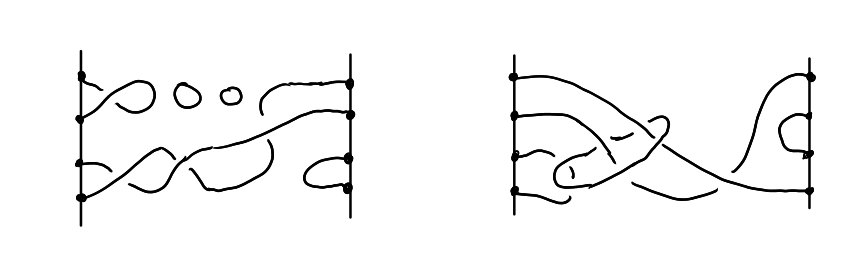
\includegraphics[scale=.25]{images/8.png}
\end{center}

We resolve any crossing using the relation 
\begin{center}
  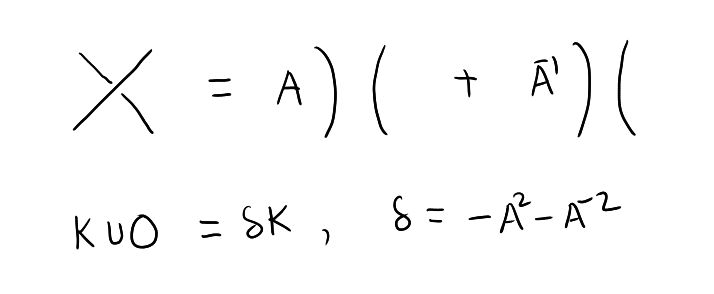
\includegraphics[scale=.25]{images/9.png}
\end{center}

  Let $A_n$ be an algebra over the ring $\mathbb{Z}[A, A^{-1}]$ of Laurent polynomials generated by the generators $U_i$ for $i = 1,\ldots, n-1$ where $U_i$ is 
  
\begin{center}
  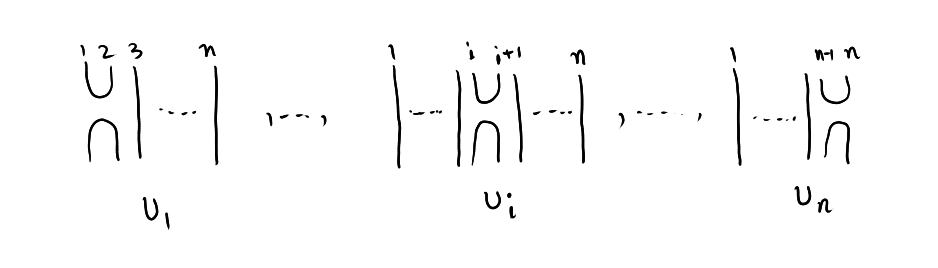
\includegraphics[scale=.25]{images/10.png}
\end{center}
  and the Jones relations 
\begin{align*}
  U_i^2 &= \delta U_i, \hspace*{1em}\text{where } \delta = -A^2-A^{-2} \\
  U_iU_{i\pm 1}U_i &= U_i, \\
  U_iU_j &= U_jU_i, \hspace*{.6em} \text{if } |i-j|>1.
\end{align*}

The Jones relations can be visualized as
\begin{center}
  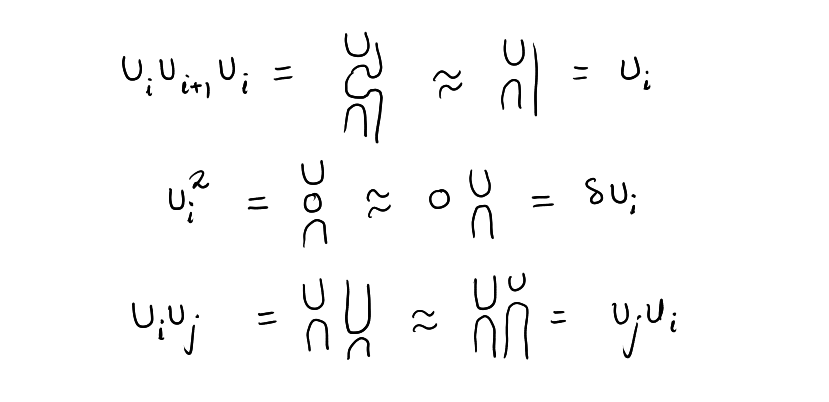
\includegraphics[scale=.25]{images/11.png}
\end{center}

A tangle $U$ can be reduced to have no crossings and no additional loops. Taking its closure (by a process similar to the closure of braids) results in a diagram of an unlink.

We define $|| U ||$ to be the number of components in the unlink minus 1.

We define $\rho_n : B_n \to A_n$ by 
\begin{align*}
  \sigma_i &\rightsquigarrow A + A^{-1}U_i, \\
  \sigma^{-1}_i &\rightsquigarrow A^{-1} + AU_i.
\end{align*}

\begin{theorem}
The map $\rho_n: B_n \to A_n$ is a representation of the Artin braid group $B_n$.
\end{theorem}
\begin{proof}
It is easily checked that $\rho_n$ preserves the braid relations. That is, 
\begin{align*}
  \rho_n(\sigma_i)\rho_n(\sigma^{-1}_n) &= 1, \\
  \rho_n(\sigma_i\sigma_{i+1}\sigma_i) &= \rho_n(\sigma_{i+1}\sigma_i\sigma_{i+1}), \\
  \rho_n(\sigma_i\sigma_j) &= \rho_n(\sigma_j\sigma_i) \text{ if } |i-j|>1.
\end{align*}
Indeed, 
\begin{align*}
  \rho_n(\sigma_i)\rho_n(\sigma_i^{-1}) &= (A+A^{-1}U_i)(A^{-1} + AU_i) \\
                                        &= 1 + (A^{-2} + A^2)U_i + U_i^2 \\
                                        &= 1 + (A^{-2} + A^2)U_i + \delta U_i \\
                                        &= 1 + (A^{-2} + A^2)U_i + (-A^{-2} - A^2)U_i \\
  &= 1,
\end{align*}
\begin{align*}
  \rho_n(\sigma_i\sigma_{i+1}\sigma_i) &= (A+A^{-1}U_I)(A + A^{-1}U_{i+1})(A + A^{-1}U_i) \\
                                       &= (A^2 + U_{i+1} + U_i + A^{-2}U_iU_{i+1})(A + A^{-1}U_i) \\
                                       &= A^3 + AU_{i+1} + AU_i + A^{-1}U_iU_{i+1} + A^{-1}U_i^2 + AU_i + A^{-1}U_{i+1}U_i + A^{-3}U_iU_{i+1}U_i \\
                                       &= A^3 + AU_{i+1} + (A^{-1}\delta + 2A)U_i + A^{-1}(U_iU_{i+1} + U_{i+1}U_i) + A^{-3}U_i \\
                                       &= A^3 + AU_{i+1} + (A^{-1}(-A^2 - A^{-2}) + 2A + A^{-3})U_i + A^{-1}(U_iU_{i+1} + U_{i+1}U_i) \\
  &= A^3 + A(U_{i+1} + U_i) + A^{-1}(U_iU_{i+1} + U_{i+1}U_i),
\end{align*}
and as we can see, the final equation is symmetric in $i$ and $i+1$, and finally 
\begin{align*}
  \rho_n(\sigma_i\sigma_j) &= \rho_n(\sigma_i)\rho_n(\sigma_{j}) \\
                           &= (A+A^{-1}U_i)(A + A^{-1}U_j) \\
                           &= (A + A^{-1}U_j)(A + A^{-1}U_i) \\
  &= \rho_n(\sigma_j\sigma_i).
\end{align*}
This completes our proof that $\rho_n$ is a representation of the braid group.
\end{proof}

\subsection{Jones polynomial}

The bracket polynomial (first introduced by Kauffman) is defined for knots and links using some skein relations. Although it is not a link invariant (it fails to be invariant under the Reidemeister move of type I), we can normalize it so that it yields the famous Jones polynomial.

We shall now derive the bracket polynomial from our representation $\rho_n$ of the braid group. Let $\beta = \sigma^{a_1}_{i_1}\cdots \sigma^{a_k}_{i_k} \in B_n$ be some braid. Then
\begin{displaymath}
\rho_n(\beta) = \prod^k_{t=1} (A+A^{-1}U_{i_t})^{a_t} = \sum_s \langle \beta | s \rangle U_s,
\end{displaymath}
where $\langle \beta | s \rangle \in \mathbb{Z}[A, A^{-1}]$ is the coefficient of $U_s$ in the expansion of $\rho_n(\beta)$.

We define $\langle U_s \rangle = \delta^{||U_s||}$ and the bracket for the closed braid $\bar{\beta}$ by 
\begin{displaymath}
\langle \bar{\beta} \rangle = \sum_s \langle \beta | t \rangle \delta^{||U_s||}.
\end{displaymath}
We have constructed a polynomial function for closed braids. This is indeed the Kauffman bracket polynomial. As we can check, it fails to be invariant under Markov moves. To make it an invariant, we have to normalize it. We define the \emph{writhe} of a braid, denoted by $w(\beta)$, to be the image of $\beta$ under the homomorphism $B_n \to \Z$ sending the generators $\sigma_i$ to $1$.

We normalize the bracket 
\begin{displaymath}
  \langle \bar{\beta} \rangle = (-A^3)^{-w(\beta)} \sum_s \langle \beta | t \rangle \delta^{||U_s||}.
\end{displaymath}
  Given an oriented link $K$ in $\mathbb{R}^3$ we define 
\begin{displaymath}
V(K) = \langle \bar{\beta} \rangle,
\end{displaymath}
where $\beta$ is a braid whose closure is isotopic to $K$.

\begin{theorem}
The polynomial $V$ is a link invariant.
\end{theorem}
  
\begin{proof}
  Let $K$ and $K^{\prime}$ be two ambient isotopic links in $\R^3$. By Alexander's theorem, we can find two braids, $\beta$ and $\beta^{\prime}$ such that $K$ (resp. $K^{\prime}$) is isotopic to the closure of $\beta$ (resp. $\beta^{\prime}$). By Markov's theorem, $\bar{\beta}$ and $\overline{\beta^{\prime}}$ are related by a sequence of Markov moves. Therefore, it suffices to show that the normalized bracket $\langle \bar{\beta} \rangle$ is invariant under Markov moves. 
\begin{enumerate}
\item\label{item:7} We first consider the possibility of equivalence in a given braid group. It is clear to us that the invariance follows directly from our construction of $\rho_n$ as a representation of the braid group. 
\item\label{item:8} For conjugation, we must show that $\langle \bar{\beta} \rangle$ for some $\alpha \in B_n$. It suffices to check that $\rho_n(\beta) = \rho_n(\alpha\beta\alpha^{-1})$. Since $\rho$ is a homomorphism, it suffices to show that $\rho_n(\beta) = \rho_n(\sigma_i\beta\sigma^{-1}_i)$. This can be checked by expansion: 
\begin{align*}
  \rho_n (\sigma_i\beta\sigma_i^{-1}) &= (A+A^{-1}U_i)\rho_n(\beta)(A^{-1} + AU_i) \\
                                      &= (A\rho_n(\beta) + A^{-1}U_i\rho_n(\beta) )(A^{-1} + AU_i) \\
                                      &= \rho_n(\beta) + (A^{-2} + A^2)U_i\rho_n(\beta) + U_i^2\rho_n(\beta) \\
                                      &= \rho_n(\beta) + (A^{-2} + A^2)U_i\rho_n(\beta) + (-A^{-2} - A^2)U_i\rho_n(\beta) \\
  &= \rho_n(\beta).
\end{align*}
\item\label{item:9} To show that the normalized bracket is invariant under $\beta \to \beta \sigma_n$, we first observe that $w(\beta \sigma_n) = w(\beta) + 1$. Then 
\begin{align*}
  \langle \overline{\beta\sigma_n}\rangle &= (-A^3)^{w(\beta) + 1} (\sum_t^{} \langle \beta | t \rangle \delta^{||U||})(A + A^{-1}\langle U_i \rangle) \\
                                          &= \langle \bar{\beta} \rangle (-A^3(A + A^{-1}\langle U_n \rangle)) \\
                                          &= \langle \bar{\beta} \rangle (-A^4 - A^2\langle U_n \rangle) \\
                                          &= \langle \bar{\beta} \rangle (-A^4 - A^2(-A^2 - A^{-2})) \\
                                          &= \langle \bar{\beta} \rangle (-A^4 + 1 + A^4) \\
  &= \langle \overline{\beta}\rangle.
\end{align*}
\end{enumerate}
This completes our proof that $V$ is an invariant for oriented links.
\end{proof}
